
\begin{frame}[fragile]
\frametitle{startActivityForResult y onActivityResult}

\textbf{¿Para qué sirven?}

\begin{itemize}
    \item Permiten iniciar una actividad esperando un resultado de regreso.
    \item Son útiles cuando se necesita que una segunda pantalla devuelva información (por ejemplo, selección de datos o confirmaciones).
\end{itemize}

\textbf{Flujo de funcionamiento:}
\begin{enumerate}
    \item Se inicia la actividad con \texttt{startActivityForResult()}.
    \item La segunda actividad procesa la información.
    \item Se devuelve un resultado mediante \texttt{setResult()}.
    \item La actividad original recibe el resultado en \texttt{onActivityResult()}.
\end{enumerate}

\textbf{Ejemplo en Java:}

%\begin{block}{Archivo \textbf{activity\_main.xml}}
\begin{minted}[linenos,fontsize=\tiny]{java}
// Lanzar actividad
Intent intent = new Intent(this, SegundaActivity.class);
startActivityForResult(intent, 1);

// Recibir resultado
@Override
protected void onActivityResult(int requestCode, int resultCode, Intent data) {
    if (requestCode == 1 && resultCode == RESULT_OK) {
        String resultado = data.getStringExtra("dato");
    }
}
\end{minted}

%\end{block}
\end{frame}


\begin{frame}{Lectura de Archivos en Android (Java)}
\textbf{Método: readFromFile(Uri uri, String text)}

\begin{itemize}
    \item Este método permite leer el contenido de un archivo a partir de una \textbf{URI}.
    \item Utiliza el \textbf{ContentResolver} para acceder a recursos externos.
\end{itemize}


\textbf{Flujo del código:}
\begin{enumerate}
    \item Se obtiene un flujo de entrada:
    \begin{itemize}
        \item \texttt{InputStream is = getContentResolver().openInputStream(uri);}
    \end{itemize}
    
    \item Se crea un lector de texto:
    \begin{itemize}
        \item \texttt{BufferedReader bf = new BufferedReader(new InputStreamReader(is));}
    \end{itemize}
    
    \item Se lee el archivo línea por línea:
    \begin{itemize}
        \item Se usa un ciclo \texttt{while} para concatenar el contenido en una variable.
    \end{itemize}
    
    \item Se muestra el contenido en pantalla:
    \begin{itemize}
        \item Se obtiene un \texttt{TextView} con \texttt{findViewById}.
        \item Se asigna el texto con \texttt{setText(FileContents)}.
    \end{itemize}
\end{enumerate}


\textbf{Manejo de errores:}
\begin{itemize}
    \item Se utiliza un bloque \texttt{try-catch} para capturar excepciones \texttt{IOException}.
\end{itemize}

\end{frame}


\begin{frame}{Escritura de Archivos en Android}
\textbf{Método: writeInFile(...)}

\begin{itemize}
    \item Este método permite escribir texto en un archivo identificado por una URI.
    \item Utiliza flujos de salida (\textit{OutputStream}) para manejar la escritura.
\end{itemize}


\textbf{Parámetros:}
\begin{itemize}
    \item \textbf{Uri uri:} Dirección del archivo donde se escribirá el contenido.
    \item \textbf{String text:} Texto que se desea guardar.
\end{itemize}


\textbf{Funcionamiento:}
\begin{itemize}
    \item Se obtiene un \textbf{OutputStream} mediante \texttt{getContentResolver()}.
    \item Se envuelve en un \textbf{BufferedWriter} para escribir texto eficientemente.
    \item Se escribe el contenido con \texttt{write(text)}.
    \item Se asegura la escritura con \texttt{flush()}.
    \item Se cierra el flujo con \texttt{close()}.
\end{itemize}


\textbf{Manejo de errores:}
\begin{itemize}
    \item Se utiliza un bloque \texttt{try-catch} para capturar excepciones de tipo \texttt{IOException}.
\end{itemize}


\end{frame}


\begin{frame}[fragile]
\frametitle{Demo 09: Lectura y Escritura de Archivos de Texto}
\begin{columns}
\column{0.80\linewidth}
Del Repositorio Github:
\begin{itemize}
\item Copiar el archivo \textit{MainActivity\_Demo09.java} (dentro del Folder códigosJAVA) al mismo directorio donde esta el MainActivity.java
\item Copiar el archivo \textit{activity\_main\_demo09.xml} (dentro del Folder Carpeta\_layout) al mismo directorio donde esta el activity\_main.xml

%\item Copiar los archivos \textit{cgup.jpg} y \textit{logo\_upv\_2019.png} localizados dentro de la folder \textit{Carpeta\_drawable} en el directorio \textit{res/drawable} del proyecto de AS.
\item Modificar en el archivo \textit{AndroidManifest.xml} la cadena \textit{.MainActivity\_Demo08} por \textit{.MainActivity\_Demo09}.
\item Ir a la linea 22 de archivo del archivo \textit{MainActivity\_Demo09.java}, poner el cursos en la palabra (en Rojo) \textit{documentfile}, presionar la combinación ALT+ENTER, y seleccionar de la lista desplegable la opcion ``Add dependency on ....''. Esto quitará el error y hara los ajustes necesarios. 
\end{itemize}

%\begin{block}{Demo \#09}
%Un App que permite escribir el contenido de un EditText a un archivo y cargar el contenido de cualquier archivo en el EditText
%\end{block}


\column{0.20\linewidth}

\begin{center}
 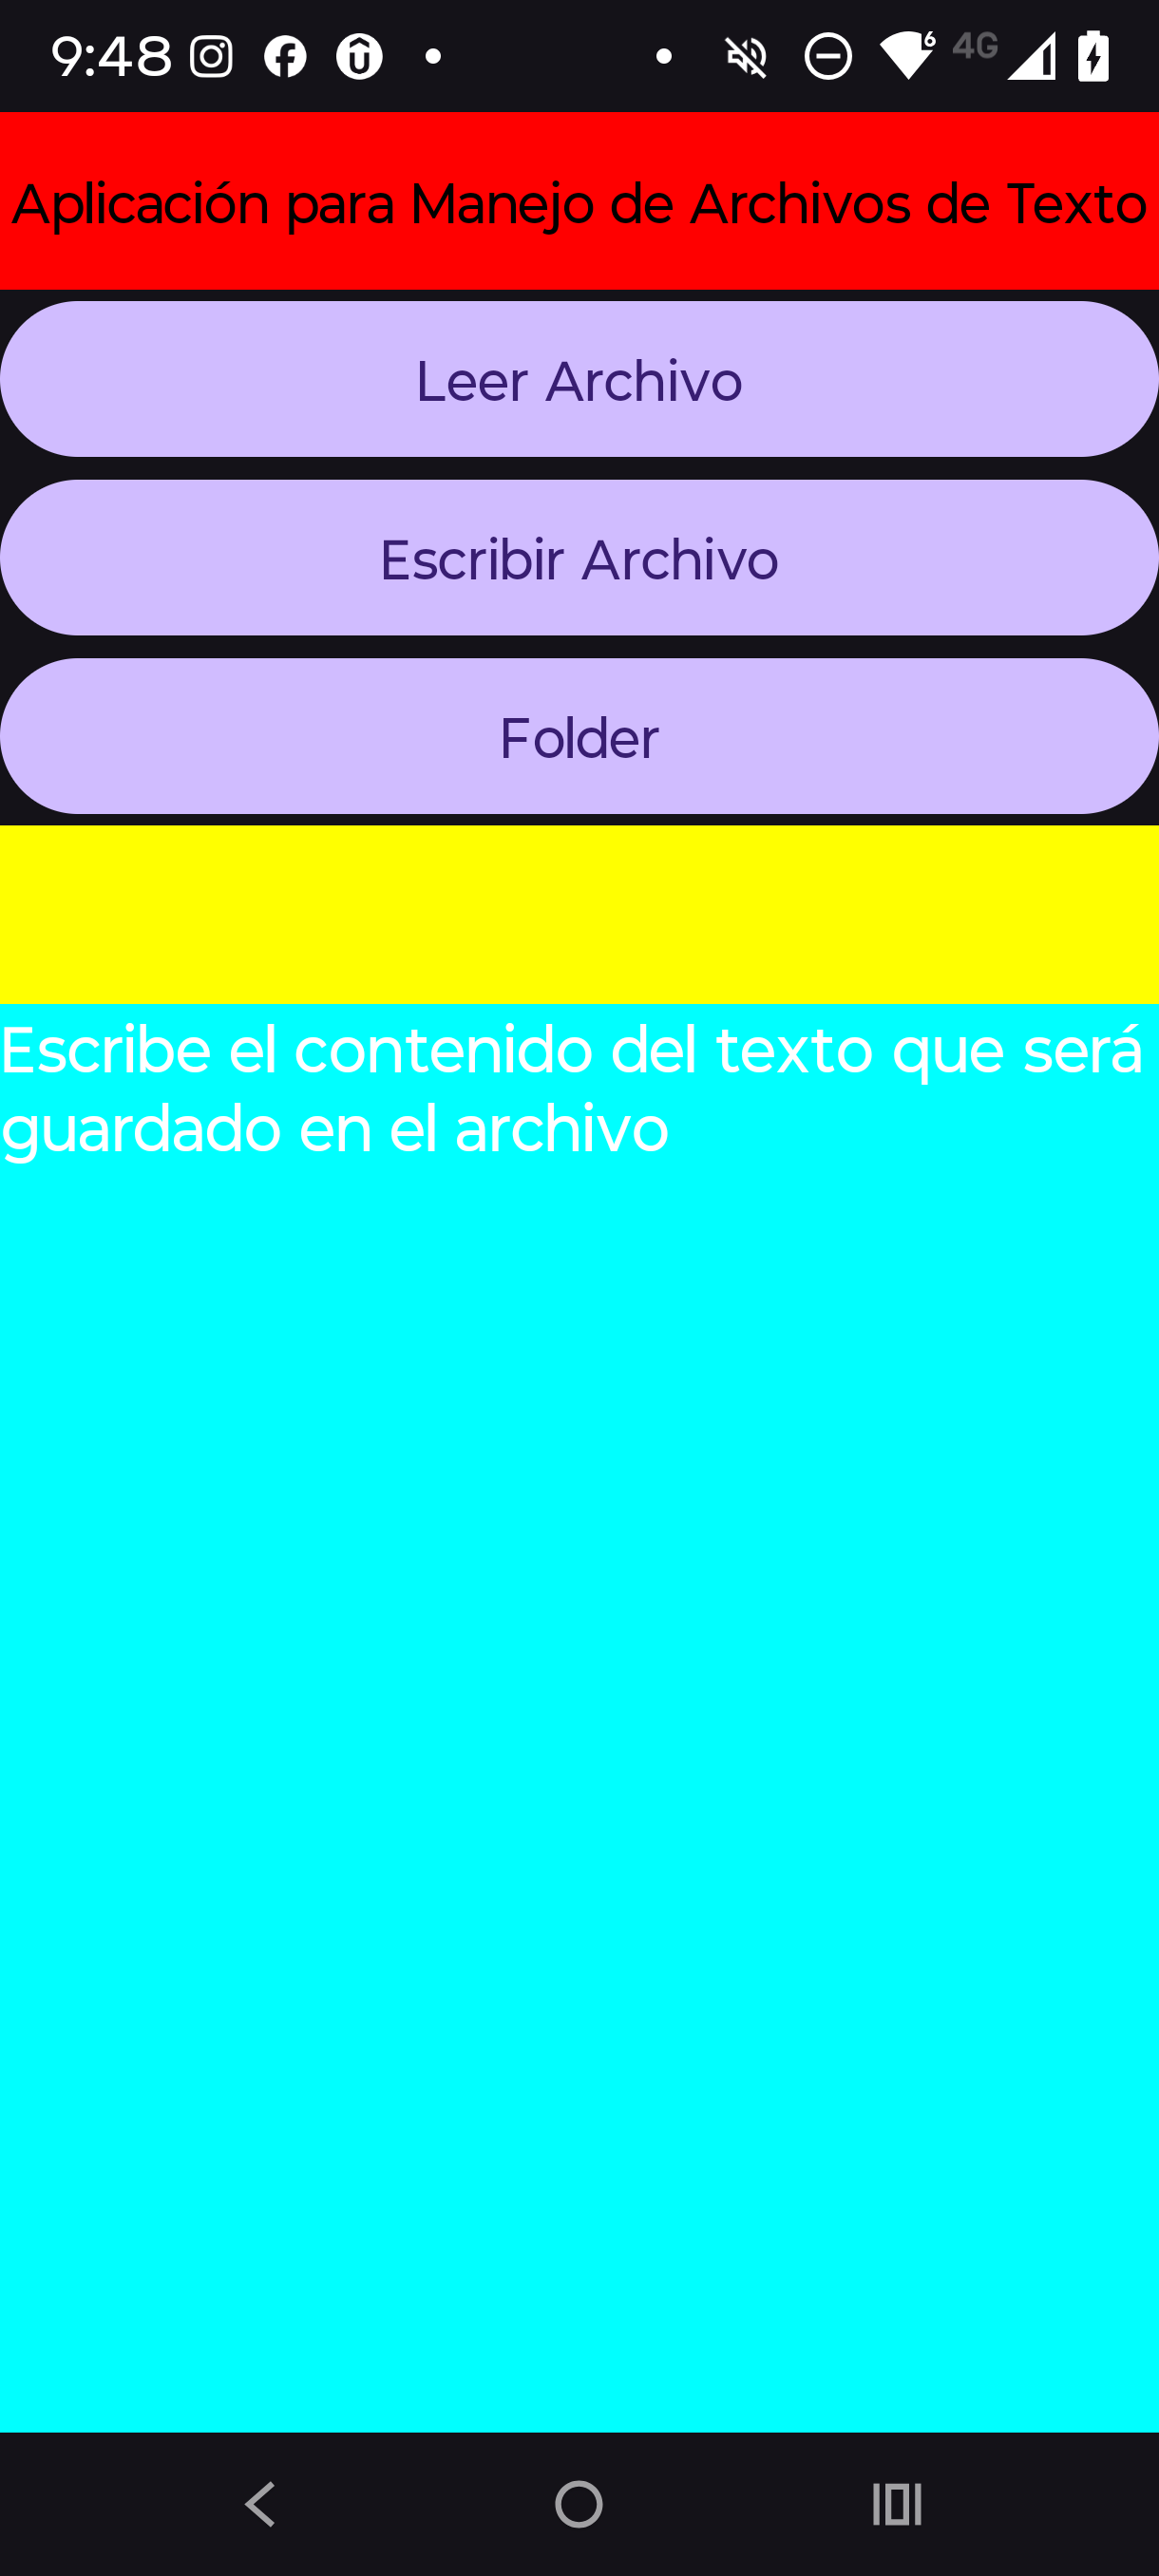
\includegraphics[width=0.98\textwidth]{02_TallerCBTis/figs/Demo09}
\end{center}

\end{columns}

\end{frame}

